%---------
% place your email id between the braces so that your homework has a name
\def\yourname{Mark Xiong}
% -----------------------------------------------------
\def\duedate{4/26/24}
\def\duelocation{via \href{https://www.gradescope.com/courses/753885}{Gradescope}}
\def\hnumber{6}
\def\prof{Lorenzo Orecchia}
\def\course{\href{https://canvas.uchicago.edu/courses/56880}{CMSC 27200 - Spring 2024}}
%-------------------------------------

\documentclass[10pt]{article}
\usepackage[colorlinks,urlcolor=blue]{hyperref}
\usepackage[osf]{mathpazo}
\usepackage{amsmath,amsfonts,graphicx}
\usepackage{latexsym}
\usepackage{subfig}
\usepackage{algpseudocode}
\usepackage[shortlabels]{enumitem}
\usepackage{algorithm}
\usepackage{listings}
%\usepackage[top=1in,bottom=1.4in,left=1.5in,right=1.5in,centering]{geometry}
\usepackage{fullpage}
\usepackage{color}
\definecolor{mdb}{rgb}{0.3,0.02,0.02} 
\definecolor{cit}{rgb}{0.05,0.2,0.45}
\usepackage{wrapfig}
%\pagestyle{myheadings}
\usepackage{tikz}
\usepackage{qtree}
\usepackage{tikz-qtree}
\markboth{\yourname}{\yourname}

\thispagestyle{empty}

\newenvironment{proof}{\par\noindent{\it Proof.}\hspace*{1em}}{$\Box$\bigskip}
\newcommand{\qed}{$\Box$}
\newcommand{\alg}[1]{\mathsf{#1}}
\newcommand{\OPT}{\mathsf{OPT}}
\newcommand{\SOL}{\mathsf{SOL}}
\newcommand{\handout}{
   \renewcommand{\thepage}{H\hnumber-\arabic{page}}
   \noindent
   \begin{center}
      \vbox{
    \hbox to \columnwidth {\sc{\course} --- \prof \hfill}
    \vspace{-2mm}
    \hbox to \columnwidth {\sc due \MakeLowercase{\duedate} \duelocation\hfill {\Huge\color{mdb}H\hnumber.\yourname}}
      }
   \end{center}
   \vspace*{2mm}
}
\newcommand{\solution}[1]{
\vspace{2mm}

\noindent Collaborators:

\vspace{5mm}

\medskip\noindent{\color{cit}\textbf{Solution:} #1}}

\newcommand{\bit}[1]{\{0,1\}^{ #1 }}
\newcommand{\extraspace}{\medskip\noindent{\color{cit} Extra space for your solution}\newpage}
%\dontprintsemicolon
%\linesnumbered=
\newtheorem{problem}{\sc\color{cit}Problem}
\newtheorem{lemma}{Lemma}
\newtheorem{theorem}{Theorem}
\newtheorem{definition}{Definition}
\newtheorem{claim}{Claim}


\begin{document}
\handout
\begin{itemize}
\item The assignment is due at Gradescope on \duedate.

\item A LaTeX template will be provided for each homework. You are strongly encouraged to type your homework into this template using \LaTeX.  If you are writing by hand, please fill in the solutions in this template, inserting additional sheets as necessary. This will help facilitate the grading.

\item You are permitted to discuss the problems with up to 2 other students in the class (per problem); however, {\em you must write up your own solutions, in your own words}. Do not submit anything you cannot explain. If you do collaborate with any of the other students on any problem, please list all your collaborators in the appropriate spaces.

\item Similarly, please list any other source you have used for each problem, including other textbooks or websites.

\item {\em Show your work.} Answers without justification will be given little credit.

\item Your homework is \textit{resubmittable}. Please refer to the course syllabus on Canvas for a more detailed description of this. For any problem that you have not changed from your last submission, please make sure to indicate this in your submission to help our graders grade faster. 

\end{itemize}

\newpage

%%%%%%%%%%%%%%%%%%%%%%%%%%%%%%%%%%%%%%%%%%%

%%%%%%%%%%%%%%%%%%%%%%%%%%%%%%%%%%%%%%%%%%%

\begin{problem}[Scenic Route] Lorenzo wants to drive from San Francisco to Chicago, taking the shortest walk he can. However, he also really wants to drive along the route that passes through Yellowstone National Park. Find the shortest walk that passes through the park. 

More formally, you are given a connected, directed, weighted graph $G=(V, E)$, where each $e \in E$ represents a different route, $w(e)$ is the length of the route $e$, and each $v \in V$ represents a points connecting some number of different routes. Furthermore, $s \in V$ represents San Francisco, and $t \in V$ represents Chicago, and there is some edge $(y_1, y_2) \in E$ representing the edge through Yellowstone that Lorenzo must take. Note that the edge $(y_2, y_1)$ may exist, but is not the route that Lorenzo wants to take.  Note also that it is possible that taking this edge forces Lorenzo to make a cycle - this is okay.

\begin{enumerate}[(a)]
    \item Provide pseudocode for an algorithm that finds the desired walk by running Dijkstra's a constant number of times. Sketch a proof of correctness. You do not need to analyze runtime, but it should not take longer than $O((|V|+|E|)\log|V|)$ (assuming a Binary heap implementation of Dijkstra's). 
    \item Describe (in words) a way to modify $G$ to make $G' = (V', E')$, such that running Dijkstra's algorithm (unmodified) a single time on $G'$ lets you find the correct walk with a linear amount of processing. Your modifications should not affect the algorithm's total asymptotic runtime. Sketch a proof of correctness, and sketch a proof that the modifications do not affect the total runtime. 
\end{enumerate}

\end{problem}

\begin{solution}
    the solution is as follows:
    \begin{enumerate}[(a)] 
        \item  \begin{algorithm}
            \caption{Scenic Route} 
            \begin{algorithmic}[1]
            \Statex \textbf{Input:} $G$, $s$, $t$, $y_1$, $y_2$
            \Statex \textbf{Output:} The shortest path from San Francisco to Chicago that passes through Yellowstone National Park
            \Statex 
            \Function{Dijkstra}{G, source} (helper function)
                \State distance = array of $\infty$ 
                \State distance[source] = 0
                \State Q = priority queue of vertices
                \State Q.add(source)
                \While{Q is not empty}
                    \State u = Q.pop() min distance in Q
                    \For{each neighbor v of u}
                        \If{distance[u] + weight(u, v) $<$ distance[v]}
                            \State distance[v] = distance[u] + weight(u, v)
                            \State Q.update(v, distance[v])
                        \EndIf
                    \EndFor
                \EndWhile

            \EndFunction
            \Statex
            \Function{RouteST}{$G$, $s$, $t$, $y_1$, $y_2$}
                \State D1 = \Call{Dijkstra}{$G$, $s$}
                \State D2 = \Call{Dijkstra}{$G$, $y_2$}
                \State ylpath = $w(y_1, y_2)$

                \State return D1[$y_1$] + ylpath + D2[$t$]
            \EndFunction
            \end{algorithmic}
        \end{algorithm}
        Proof of correctness: Dijkstra's algorithm guarantees that the shortest path from a single source to any other vertex in a graph with non-negative weights is found.
        By running Dijkstra's algorithm twice, we can find the shortest path from San Francisco to $y_1$ and from $y_2$ to Chicago. The algorithm calculates the shortest path that passes through the yellow stone edge by 
        combining the two shortest paths and the weight of the yellow stone edge. The two calls to Dijkstra's algorithm guarantee that the shortest path is found.
        \item Introduce a negative weight to the edge going from $y_1$ to $y_2$, the negative value should ensure it's sufficient to overcome any other potentially shorter paths that do not include $e(y_1, y_2)$, but not so large as to cause numerical underflows or unintended consequences in the algorithm.  
        \\ \\
        Proof of Correctness: This change in weight of $e(y_1, y_2)$ ensures Dijkstra's algorithm includes this edge as it selects paths based on the lowest cumulative weight. Moreover, since we preserve the original weights of the other edges, the route still takes shortest path from $s$ to $y_2$, and $y_2$ to $t$, the shortest path is still found.
        \\ \\
        Proof of Preserved-Runtime: As we only changed a weight on an edge, the number of edges $|E|$ and $V$ vertices do not change. The time complexity is driven by the operations of the priority queue, which are determined by the number of edges and vertices. The runtime is not affected by the change in weight.

    \end{enumerate}


\end{solution}
\newpage

%%%%%%%%%%%%%%%%%%%%%%%%%%%%%%%%%%%%%%%%%%%

%%%%%%%%%%%%%%%%%%%%%%%%%%%%%%%%%%%%%%%%%%%

\begin{problem}[Homecoming]
Billy gets lost easily, so every time he goes anywhere in town, he has to stop by home first to check in. With that in mind, he wants a new understanding of how ``far" locations in town are from each other. 

The town is modeled by a connected, weighted, directed graph $G=(V, E)$, and you are given some home vertex $h \in V$. Billy wants the matrix $M$ of size $n \times n$, where 
\[ 
    M[v, u] = \text{length of shortest walk from }v\text{ to }u \text{ that contains }h.
\]
Even the entry $M[v, v]$ must correspond to a walk containing $h$.

Provide pseudocode, a formal proof of correctness, and a formal proof of runtime for an algorithm that outputs this matrix. For full credit your algorithm should run in time $O(|V|^2)$. You may assume that $|E| = O(|V|)$. 
\end{problem}

\begin{solution}
    The solution is as follows:
    \begin{algorithm}
        \caption{Homecoming} 
        \begin{algorithmic}[1]
        \Statex \textbf{Input:} $G$, $h$
        \Statex \textbf{Output:} The matrix $M$ of size $n \times n$ where $M[v, u]$ is the length of the shortest walk from $v$ to $u$ that contains $h$
        \Statex 
        \Function{Dijkstra}{G, source} (helper function)
            \State distance = array of $\infty$ 
            \State distance[source] = 0
            \State Q = priority queue of vertices
            \State Q.add(source)
            \While{Q is not empty}
                \State u = Q.pop() min distance in Q
                \For{each neighbor v of u}
                    \If{distance[u] + weight(u, v) $<$ distance[v]}
                        \State distance[v] = distance[u] + weight(u, v)
                        \State Q.update(v, distance[v])
                    \EndIf
                \EndFor
            \EndWhile

        \EndFunction
        \Statex
        \Function{Homecoming}{$G$, $h$}
            \State $G'$ = reverse all edges in $G$
            \State DFromH = \Call{Dijkstra}{$G$, $h$}
            \State DToH = \Call{Dijkstra}{$G'$, $h$}
            \State M = matrix of size $|V| \times |V|$
            \For {each vertex $v$ in $V$}
                \For {each vertex $u$ in $V$}
                    \State M[v, u] = DToH[v] + DFromH[u]
                \EndFor
            \EndFor

            \State return $M$
        \EndFunction
        \end{algorithmic}
    \end{algorithm} \\
    Proof of correctness:  The algorithm is based on on the principle that any shortest path from vertex $
    v$ to vertex $u$ that must pass through a third vertex $h$ can be decomposed into two distinct shortest paths: $v$ to $h$ and $h$ to $u$. This decomposition is valid due to the nature of shortest paths in graphs with non-negative weights.
    Running Dijkstra's algorithm from $h$ on the graph $G'$ with all edges on $G$ reversed, we can find the shortest path to $h$ from any vertex in $G$. Similarly, running Dijkstra's algorithm from $h$ on the original graph $G$, we can find the shortest path from $h$ to any vertex in $G$. 
    By summing the two shortest paths, we can find the shortest path from any vertex $v$ to any vertex $u$ that passes through $h$. The final matrix $M[v, u]$ is constructed with loops that each iteration finds the shortest path from $v$ to $u$ that passes through $h$. The correctness of this matrix 
    directly comes from the correctness of Dijkstra's algorithm. \\
    \\
    Proof of runtime: The algorithm runs Dijkstra's algorithm twice, once on the original graph $G$ and once on the reversed graph $G'$. The runtime of Dijkstra's algorithm using a binary heap is $O((|V|+|E|)\log|V|)$. Since $|E| = O(|V|)$, the runtime of Dijkstra's algorithm is $O(|V|\log|V|)$. The loops that construct the matrix $M$ have a runtime of $O(|V|^2)$. The total runtime of the algorithm is $O(|V|^2) + O(|V|\log|V|) + O(|V|\log|V|) = O(|V|^2)$.
\end{solution}

\newpage

%%%%%%%%%%%%%%%%%%%%%%%%%%%%%%%%%%%%%%%%%%%

%%%%%%%%%%%%%%%%%%%%%%%%%%%%%%%%%%%%%%%%%%%
\begin{problem}[Colorful MST]
    You are given access to a program $P$ to find the MST of a weighted undirected graph with any edge weights. However you are now given as input a weighted undirected graph and some edges are colored red while the others are blue. You further know that all the edge weights in the input given to you are integers. Design an algorithm that takes only $O(|V|+|E|)$ additional time, \textbf{apart from the time taken in a single call to $P$}, to output a MST of your input graph that uses as few red edges as possible. Note that \textbf{you still want to output a minimum cost spanning tree}; so the goal is to minimize the total weight, but of the many possible spanning trees that minimize the weight, you want one that uses as few red edges as possible. Prove the correctness of your algorithm.
\end{problem}
\begin{solution}
    The solution is as follows:
    \begin{algorithm}
        \caption{Colorful MST} 
        \begin{algorithmic}[1]
        \Statex \textbf{Input:} $G$, $P$
        \Statex \textbf{Output:} A MST of the input graph that uses as few red edges as possible
        \Statex 
        \Function{ColorfulMST}{$G$, $P$}
            \State $\epsilon$ = $1 \times 10^{-10}$
            \For {each edge $e$ in $G$}
                \State weight$(e) += \epsilon$ if $e$ is red
            \EndFor
            \State $MST$ = $P(G)$ 
            \Return $MST$
        \EndFunction
        \end{algorithmic}
    \end{algorithm} \\
    Proof of correctness: The algorithm works by adding a small value $\epsilon$ to the weight of each red edge in the graph. By adding this small value, the algorithm ensures that the MST algorithm $P$ will preferentially select blue edges over red edges in cases where weights of two edges of different colors tie together.
     Since the MST algorithm $P$ is guaranteed to find the minimum cost spanning tree, the algorithm will select the MST that uses as few red edges as possible as blue edges are relatively lighter with added $\epsilon$ on red edges.
     The MST computed still adheres to the minimum weight principle because $\epsilon$ is too small to affect the selection of edges unless there's a tie by original weight. Thus, the tree remains optimal in terms of weight while minimizing red edges.
\end{solution}

\newpage
%%%%%%%%%%%%%%%%%%%%%%%%%%%%%%%%%%%%%%%%%%%

%%%%%%%%%%%%%%%%%%%%%%%%%%%%%%%%%%%%%%%%%%%

\begin{problem}[Huffman Coding]
A geneticist wants to encode a genetic sequence, and plans to use Huffman Coding to do so. 
\begin{enumerate}[(a)]
    \item Say the nucleotides A, C, G, T appear in the sequence with frequencies 31\%, 20\%, 9\%, 40\% respectively. What is the Huffman encoding of these four characters?
    \item The geneticist is an alien geneticist, and these extraterrestrial species have $n$ different nucleotides in their genes. If the geneticist encoded their sequences, what is the longest possible code word? Provide a set of frequencies that achieves this legnth.  
    \item Find the largest value $p$ such that, if all nucleotide frequencies are less than $p\%$, codewords are \textit{guaranteed} to not have length $1$. Sketch a proof.
\end{enumerate}

\end{problem}

\begin{solution}
    The solution is as follows:
    \begin{enumerate}[(a)]
        \item The Huffman encoding of the four characters looks like the following:
        \begin{figure}[ht]
            \centering
                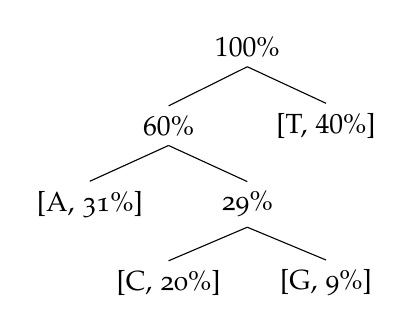
\begin{tikzpicture}[level distance=1cm,
                                    level 1/.style={sibling distance=2cm},
                                    level 2/.style={sibling distance=2cm}]
                    \node {$100\%$}
                        child {node {$60\%$}
                            child {node {[A, 31\%]}}
                            child {node {29\%}
                                child {node {[C, 20\%]}}
                                child {node {[G, 9\%]}}}            
                        }
                        child {node{[T, $40\%$]}};
                \end{tikzpicture}
                \caption{Huffman encoding of A, C, G, T}
        \end{figure}
        \item The longest possible code word is $n-1$. One senario that achieves this is as follows:
        \begin{itemize}
            \item The most frequent nucleotide has frequency of 50\%
            \item The second most frequent nucleotide has frequency of 25\%
            \item The third most frequent nucleotide has frequency of 12.5\%
            \item Continue halving the frequency of the nucleotide until the last nucleotide has frequency of $1/2^n\%$
        \end{itemize}
        \item The largest value $p$ is $33.333\%$ or $\frac{1}{3}$. We could prove by contradiction. Assume that we have a full binary tree that does not have a codeword of length 1. This implies the root of the tree will have no direct frequencies as its children.
        As the largest frequency is no more than $\frac{1}{3}$, the other child would have a frequency greater than $\frac{2}{3}$, and its children would have a frequency greater or equal to $\frac{1}{3}$, which violates the contradiction. 
    \end{enumerate}
\end{solution}


\end{document}